\documentclass[journal]{IEEEtran}

\ifCLASSINFOpdf
  \usepackage[pdftex]{graphicx}
\else
\fi

\begin{document}
\title{Re-configurable Data Stream Processor}
\author{Baiqing Lyu \\Boston University}
\maketitle

\begin{abstract}
This document lays out the inspiration for a scalable data stream processor.
It is a general framework for data stream processing, which can be used to
build a wide variety of data processing applications. The uniqueness of this
framework is that it is designed to be scalable, and it is designed to be used
in a distributed environment.
\end{abstract}

\section{Introduction}

\IEEEPARstart{T}{he} current state of the art in data stream processing is software 
frameworks like Apache Flink, Apache Spark, and Apache Storm. These frameworks all require 
in some capacity a centralized component in its data pipeline. That often leads to a potential
single point of failure or ease of congestion that creates bottlenecks during production. The idea
is to create a stream processor that has a certain tradeoff which can be expressed of having a bit higher
latency than systems like Apache Flink, but lower than Apache Spark, including better scalability than those
frameworks in addition to having capabilities for re-configuration.

\hfill March 31, 2022

\section{Requirements}
Being able to scale up and down without downtime is a fundamental requirement for 
this data stream processor. In addition, the processor should be decentralized in 
its workers and enable fast failure recovery if a node were to suddenly disconnect.
It would also need to deliver \textbf{at least once} processing guarantees when 
ingesting incoming data. Current scope is to focus on the feasibility of a data 
stream processor that can be used in a distributed environment.
\section{Goals}
1. Create MVP of a distributed networks that allow nodes to come in and out of the 
network.

2. Give the ability to input data into the dataflow and have a sink that can recieve 
the output.

3. Develop a MVP of a data stream processor that can support easy map reduce operations 
(i.e. wordcount)
\section{Software Design}

The dataflow network design is inspired by Chord, an implementation of a distributed hash table(DHT). 
Chord creates a ring structure for the nodes and provies the ability to map a given key to some node.

As the Chord protocol supports the operation of load balancing in addition to mapping keys to nodes and controlling
the behavior when the nodes are down, it is very helpful as the baseline for the data stream processor.
The usage of finger tables within Chord provides a robust way to handle arbritrary node failures. In addition,
this can also handle the scale up and down of nodes within the processor.

The main purpose of Chord is very simple in its mission, \textit{provided a key, the protocol will
return the node that is responsible for the key}. We use this property to back state operators so that
when workers enter the ring or unexpectedly leaves, the state is still preserved and can be recovered.

\section{Map Reduce Modifications}
On top of the existing Chord implementation, we will modify it 
to support the map reduce functionality. Instead of the traditional setting
of value to a node, there will be new methods that act as operators. For example
instead of \texttt{setValue(value)} and letting Chord handle the corresponding node,
we will have \texttt{sumOperator(value)} and let Chord set the value, and instruct the
node to perform the sum operation. Similarly, we could have custom operators to perform
any actions needed, as it will be chained as a secondary set to after storing the data in their
corresponding nodes.

\section{Result sink}
The result sink is a new sink that will be used to store the results of the map reduce operation. Since
we want to minimize the need for network activity, all results will be fed into a single node. This node
will be known as the \texttt{sink node}, and will be responsible for storing the results. This node does
not participate within the ring, and can be seen as a seperate entity that is soley responsible for accepting
results and perform de-duplication and aggregation. This part of design is currently in its infant stage, as
having a single node responsible for result inherently introduces risk of failure.

In addition to an independent result sink, there is also a per node independent sink that could be used
if the data does not need to be aggregated or de-duplicated. This would then resolve the single point of
failure issue and allow for a more robust sinking mechanism for the stream processor.

\section{Data flow topology}

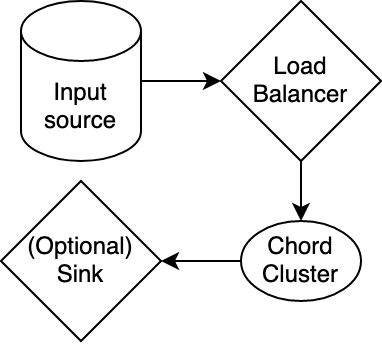
\includegraphics[scale=0.4]{topology}

\end{document}